\date{}
\title{}
\date{}
\usepackage{pgfplots}
\pgfplotsset{compat=1.16}
\usepgfplotslibrary{fillbetween}
\usetikzlibrary{patterns}
\begin{document}
\begin{frame}
    \titlepage
\end{frame}

\input{../common/listingsLib}
\usetikzlibrary{circuits.logic.mux}
\makeatletter
\pgfdeclareshape{myregister}%
{
    \inheritsavedanchors[from=rectangle]
    \inheritanchorborder[from=rectangle]
    \inheritanchor[from=rectangle]{center}
    \inheritanchor[from=rectangle]{north}
    \inheritanchor[from=rectangle]{south}
    \inheritanchor[from=rectangle]{west}
    \inheritanchor[from=rectangle]{east}
    \inheritanchor[from=rectangle]{north east}
    \inheritanchor[from=rectangle]{north west}
    \inheritanchor[from=rectangle]{south east}
    \inheritanchor[from=rectangle]{south west}
    \inheritbackgroundpath[from=rectangle]
    \saveddimen{\halfbaselength}{%
         \pgf@x=0.5\wd\pgfnodeparttextbox
         % get xsep
         \pgfmathsetlength\pgf@xc{\pgfkeysvalueof{/pgf/inner xsep}}%
         \advance\pgf@x by \pgf@xc%
         % get \ht of textbox, add to baselength 
         \advance\pgf@x by \wd\pgfnodeparttextbox
         % get minimum width
         \pgfmathsetlength\pgf@xb{\pgfkeysvalueof{/pgf/minimum width}}%
         \divide\pgf@xb by 2
         \ifdim\pgf@x<\pgf@xb%
             % yes, too small. Enlarge...
             \pgf@x=\pgf@xb%
         \fi%
     }
    \backgroundpath{
        \pgfpathrectanglecorners{\southwest}{\northeast}
        \southwest \pgf@xa=\pgf@x \pgf@ya=\pgf@y 
        \pgf@yb=\pgf@ya
        \northeast \pgf@xb=\pgf@x %\pgf@yb=\pgf@y
        \pgf@xc = \pgf@xa
        \advance\pgf@xc by \halfbaselength
        \pgf@yc=\pgf@ya
        \advance\pgf@yc by \halfbaselength
        \pgfpathmoveto{\pgfpoint{\pgf@xa}{\pgf@ya}}
        \pgfpathlineto{\pgfpoint{\pgf@xc}{\pgf@yc}}
        \pgfpathlineto{\pgfpoint{\pgf@xb}{\pgf@yb}}
        \pgfpathclose
    }
}
\makeatother

\usetikzlibrary{arrows.meta}
\usetikzlibrary{fit}

\providecommand{\cpuset}{
\tikzset{
    box/.style={draw,very thick,align=center},
    cache/.style={box,fill=yellow!20,minimum width=2cm,minimum height=1.5cm},
    regfile/.style={box,fill=blue!20,minimum height=3cm,align=center},
    alu/.style={box,fill=violet!20,minimum height=1.5cm,minimum width=2cm},
    pc/.style={box,myregister,label={center:PC},minimum height=2cm,minimum width=.75cm,fill=yellow!30},
    connect/.style={draw,ultra thick,-Latex},
}
}
\providecommand{\cpucomponent}{
\node[pc] (pc) {};
\node[cache,anchor=west] (icache) at ([xshift=1cm]pc.east) {I\$};
\node[anchor=north,box,font=\small] (ilen) at ([yshift=-.25cm]icache.south) {+ instr\\len};
\node[regfile,anchor=north west] (regfile) at ([yshift=.5cm,xshift=1cm]icache.east) {register\\file};
\node[alu,anchor=west] (math) at ([xshift=1cm]regfile.east |- pc.east) {math};
\node[cache,anchor=west] (dcache) at ([xshift=1cm,yshift=-1cm]math.east) {D\$};
\node[anchor=north,font=\small] at ([yshift=-.1cm]regfile.north) {read};
\node[anchor=south east,font=\small] at ([yshift=.25cm]regfile.south east) {write};
}
\providecommand{\cpuconnect}{
\draw[connect] (pc) -- (icache);
\draw[connect] (pc.east) -- ++(0.5cm,0cm) |- (ilen.west);
\draw[connect] (ilen.east) -- ++(0.25cm,0cm) |- ([yshift=-1.5cm,xshift=-.5cm]pc.south west) |- (pc.west);
\coordinate (pre pc) at ([xshift=-.5cm,yshift=-1.5cm]pc.west);

\draw[connect] ([yshift=-.25cm]icache.north east) -- ([yshift=-.25cm]math.north west)
    coordinate[midway] (decode middle top) coordinate (math in top);
\draw[connect] ([yshift=-1cm]icache.north east) |- ([yshift=-1cm]icache.north east -| regfile.west) coordinate (regfile read in);

\draw[connect] ([yshift=-1cm]icache.north east -| regfile.east) coordinate (regfile read out) -- ([yshift=-1cm]math.north west) coordinate (reg to math);
\draw[connect] ([yshift=.5cm]math.south east) coordinate (math out 2) -- ([yshift=.5cm]math.south east -| dcache.west) coordinate (math to cache);
\draw[connect] ([yshift=-.5cm]math.north east) coordinate (math out 1) -- ([yshift=-.5cm,xshift=.75cm]math.north east -| dcache.east)
    |- ([xshift=.75cm,yshift=-.5cm]dcache.south east) -- ([yshift=-.5cm]dcache.south -| regfile.east);
\coordinate (memory top) at ([yshift=1cm]dcache.north);
\draw[connect] (dcache.east) -- ++(0.35cm,0cm) |- ([yshift=-.25cm]dcache.south -| regfile.east)
    coordinate (regfile write in);
\coordinate (regfile write in opposite) at (regfile write in -| regfile.west);
}

\providecommand{\stagestyles}{
\tikzset{
    stage/.style={draw,line width=1mm,opacity=0.7,fill opacity=0.2},
    fetch/.style={draw=yellow,fill=yellow},
    decode/.style={draw=orange,fill=orange},
    execute/.style={draw=green,fill=green},
    memory/.style={draw=blue,fill=blue},
    writeback/.style={draw=violet,fill=violet},
    fd reg/.style={draw=yellow!50!orange,fill=yellow!30!orange!30},
    de reg/.style={draw=orange!50!green,fill=orange!30!green!30},
    em reg/.style={draw=green!50!blue,fill=green!30!blue!30},
    mw reg/.style={draw=blue!50!violet,fill=blue!30!violet!30},
}
}
\providecommand{\stageboxes}{
    \node[stage,fetch,fit=(icache) (ilen),label={north:fetch}] (fetch) {};
    \node[stage,decode,fit=(regfile read in) (regfile read out) (decode middle top),label={north:decode}] (decode) {};
    \node[stage,execute,fit=(math in top) (math),label={north:execute}] (execute) {};
    \node[stage,memory,fit=(dcache) (memory top),label={north:memory}] (memory) {};
    \node[stage,writeback,fit=(regfile write in) (regfile write in opposite) (regfile.south),label={south:writeback}] (writeback) {};
}
\providecommand{\stageregs}{
    \node[draw,myregister,anchor=north,very thick,minimum width=0.1cm,minimum height=2cm,fd reg] (fd reg) at ([xshift=.25cm,yshift=0.25cm]fetch.north east) {};
    \node[draw,myregister,anchor=north,very thick,minimum width=0.1cm,minimum height=2cm,de reg] (de reg) at ([xshift=.25cm,yshift=0.25cm]decode.north east) {};
    \node[draw,myregister,anchor=north,very thick,minimum width=0.1cm,minimum height=3cm,em reg] (em reg) at ([xshift=.25cm,yshift=0.25cm]execute.north east) {};
    \node[draw,myregister,anchor=north,very thick,minimum width=0.1cm,minimum height=1cm,mw reg] (mw reg) at ([xshift=.5cm,yshift=0.25cm]writeback.north east) {};
}
\newsavebox{\pipeCpuBox}
\savebox{\pipeCpuBox}{%
    \begin{tikzpicture}
    \cpuset
    \cpucomponent
    \cpuconnect
    \stagestyles
    \stageboxes
    \stageregs
    \end{tikzpicture}%
}



\begin{frame}
\frametitle{last time}
    \begin{itemize}
        \item cryptographic hashes; DH-like key agreement
        \item TLS handshake
            \begin{itemize}
            \item asymmetric to setup symmetric; signatures over key share
            \end{itemize}
        \item adding pipelining to single-cycle processor (laundry analogy)
        \item diminishing returns (pipeline registers, uneven split)
        \item hazard = pipeline computes wrong answer without fixes
        \item stalling (insert nops) to resolve data hazard
            \begin{itemize}
            \item wait long enough that register read happens same time/after write
            \end{itemize}
    \end{itemize}
\end{frame}

\section{challenge: hazards}

\subsection{data hazards intro}

\subsection{control hazards}
\usetikzlibrary{fit,matrix}

\begin{frame}[fragile,label=ControlFlowExample]{control hazard}
\begin{lstlisting}
cmpq %r8, %r9
je   0xFFFF
addq %r10, %r11
\end{lstlisting}
\begin{tikzpicture}
\matrix[tight matrix,nodes={text width=1cm,font=\scriptsize\tt},
        column 9/.append style={nodes={text width=1.8cm}},
        column 5/.append style={nodes={text width=0.8cm}},
        column 6/.append style={nodes={text width=2.2cm}},
        column 8/.append style={nodes={text width=0.8cm}},
        row 1/.append style={nodes={font=\scriptsize}},
        row 2/.append style={nodes={font=\scriptsize}},
        ] (tbl) {
 \& |[fill=yellow!10!white,align=center]| fetch \& rA \& rB  \& R[rA] \& R[rB] \& result \& \ldots \& \ldots \&\ldots  \\
cycle \& PC \& rA \& rB \& R[rA] \& R[rB] \& result \& \ldots \& \ldots \& \ldots \\
0 \& 0x0  \\
1 \& 0x2 \& 8  \& 9   \\ 
2 \& ??? \& --- \& --- \& 800  \& 900 \\
2 \& ??? \& --- \& --- \& --- \& --- \& less than \& ~ \& ~ \& ~ \\
};
\begin{scope}[every node/.style={draw,inner sep=0pt},
              every label/.style={font=\scriptsize,draw=none}]
    \node[fit=(tbl-1-3) (tbl-1-4),fill=yellow!50!orange!10!white,label={center:fetch$\rightarrow$decode}] {};
    \node[fit=(tbl-1-5) (tbl-1-6),fill=orange!50!green!10!white,label={center:decode$\rightarrow$execute}] {};
    \node[fit=(tbl-1-7) (tbl-1-8),fill=green!50!blue!10!white,label={center:execute$\rightarrow$writeback}] {};
    \node[fit=(tbl-1-8) (tbl-1-9),fill=blue!50!violet!10!white,label={center:execute$\rightarrow$writeback}] {};
\end{scope}
\begin{visibleenv}<2->
    \node[line width=2pt,draw,red,fit=(tbl-5-2),
          label={-45:{\tt 0xFFFF} if R[8] = R[9]; {\tt 0x12} otherwise}] {};
\end{visibleenv}
\end{tikzpicture}
\end{frame}

%\begin{frame}[fragile,label=ControlFlowExampleStall]{control hazard: stall}
%\begin{lstlisting}
%cmpq %r8, %r9
%// insert two nops
%je   0xFFFF
%addq %r10, %r11
%\end{lstlisting}
%\begin{tikzpicture}
%\matrix[tight matrix,nodes={text width=1cm,font=\scriptsize\tt},
%        column 9/.append style={nodes={text width=1.8cm}},
%        column 5/.append style={nodes={text width=0.8cm}},
%        column 8/.append style={nodes={text width=0.8cm}},
%        row 1/.append style={nodes={font=\scriptsize}},
%        row 2/.append style={nodes={font=\scriptsize}},
%        ] (tbl) {
% \& |[fill=yellow!10!white,align=center]| fetch \& rA \& rB  \& R[srcA] \& R[srcB] \& dstE \& next R[dstE] \& dstE \\
%cycle \& PC \& rA \& rB \& R[rA] \& R[rB] \& rB \& result \& rB \& result \& rB \\
%0 \& 0x0   \\
%1 \& 0x2*  \& 8  \& 9   \\ 
%2 \& 0x2*  \& 0xF  \& 0xF   \& 800  \& 900 \& 9 \\
%3 \& 0x2   \& 0xF  \& 0xF   \& --- \&  --- \& 0xF  \& 1700 \& 9 \\
%4 \& 0x10  \& 0xF  \& 0xF   \& --- \&  --- \& 0xF  \& ---  \& 0xF \\
%5 \&       \& 10  \& 11   \& --- \&  --- \& 0xF  \& ---  \& 0xF \\
%6 \&       \&     \&   \& 1000 \&  1100 \& 11 \& ---  \& 0xF \\
%};
%\begin{scope}[every node/.style={draw,inner sep=0pt},
%              every label/.style={font=\scriptsize,draw=none}]
%    \node[fit=(tbl-1-4) (tbl-1-5),fill=yellow!50!orange!10!white,label={center:fetch$\rightarrow$decode}] {};
%    \node[fit=(tbl-1-6) (tbl-1-8),fill=orange!50!green!10!white,label={center:decode$\rightarrow$execute}] {};
%    \node[fit=(tbl-1-9) (tbl-1-10),fill=green!50!blue!10!white,label={center:execute$\rightarrow$writeback}] {};
%\end{scope}
%\foreach \x/\base in {all:2/4,all:2/5,all:3/6} {
%    \begin{pgfonlayer}{bg}
%    \begin{visibleenv}<\x>
%        \pgfmathtruncatemacro{\fetchR}{\base}
%        \pgfmathtruncatemacro{\decodeR}{\base+1}
%        \pgfmathtruncatemacro{\executeR}{\base+2}
%        \pgfmathtruncatemacro{\writebackR}{\base+3}
%        \foreach \nd in {tbl-\decodeR-4,tbl-\decodeR-5,
%                         tbl-\executeR-6,tbl-\executeR-7,tbl-\executeR-8,
%                         tbl-\writebackR-9,tbl-\writebackR-10} {
%            \node[fit=(\nd),inner sep=0pt,fill=green,opacity=0.3] {};
%         }
%    \end{visibleenv}
%    \end{pgfonlayer}
%}
%\begin{visibleenv}<all:2>
%\node [fit=(tbl-4-2) (tbl-5-2), red, line width=2pt, draw, rounded corners,
%    label={[draw,fill=white,inner sep=1pt,line width=2pt]45:wait for two cycles for addq to update SF/ZF}] {};
%\end{visibleenv}
%\begin{visibleenv}<all:3>
%\node [fit=(tbl-6-2), red, line width=2pt, draw, rounded corners,
%    label={[draw,fill=white,inner sep=1pt,line width=2pt]45:execute je instruction (use SF/ZF)}] {};
%\end{visibleenv}
%\end{tikzpicture}
%\end{frame}
%
 % FIXME: correct

\subsubsection{idea: branch prediction}

\begin{frame}[fragile,label=makingGuesses]{making guesses}
\begin{lstlisting}
        subq   %rcx, %rax
        jne    LABEL
        xorq   %r10, %r11
        xorq   %r12, %r13
        ...
LABEL:  addq   %r8, %r9
        movq %r10, 0(%r11)
\end{lstlisting}
\begin{itemize}
    \item speculate: \myemph{jne} will goto LABEL
    \item right: 2 cycles faster!
    \item wrong: forget before execute finishes
\end{itemize}
\end{frame}
\begin{frame}[fragile,label=jCCYes]{jXX: speculating right}
\begin{tikzpicture}
    \matrix[tight matrix,matrix stages,
        nodes={text width=2cm,minimum height=0.5cm,text depth=.1ex,font=\small},
        column 1/.append style={nodes={text width=.8cm}},
        column 2/.append style={nodes={text width=2.2cm}},
        column 3/.append style={nodes={text width=1.8cm}},
        column 4/.append style={nodes={text width=2.6cm}},
        column 5/.append style={nodes={text width=2.0cm}},
        column 6/.append style={nodes={text width=1.8cm}}] (timeline) {
        time \& fetch \& decode \& execute \& memory \& writeback \\
        1    \& subq   \\
        2    \& jne \& subq \\
        3    \& addq [?] \& jne \& subq (set ZF) \\
        4    \& movq [?] \& addq [?] \& jne (use ZF) \& OPq \\
        5    \& movq \& movq \& addq \& jne (done) \& OPq \\
    };
    \node[anchor=south west] at ([yshift=.25cm]timeline.north west) {
\begin{lstlisting}[style=small]
        subq %r8, %r8
        jne LABEL
        ...

LABEL:  addq %r8, %r9
        movq %r10, 0(%r11)
        movq $1, %r11
\end{lstlisting}
    };
    \tikzset{every label/.style={opacity=1.0,fill=white,inner sep=2pt}}
    \begin{visibleenv}<2>
        \node[fit=(timeline-4-2),hiBox] {};
        \node[fit=(timeline-5-2) (timeline-5-3),hiBox,label={[fill=white,draw,thick]east:were waiting/nothing}] {};
    \end{visibleenv}
\end{tikzpicture}
\end{frame}

\begin{frame}[fragile,label=jCCNo]{jXX: speculating wrong}
\begin{tikzpicture}
    \matrix[tight matrix,matrix stages,
        nodes={text width=2cm,minimum height=0.5cm,text depth=.1ex,font=\small},
        column 1/.append style={nodes={text width=.8cm}},
        column 2/.append style={nodes={text width=2.2cm}},
        column 3/.append style={nodes={text width=1.8cm}},
        column 4/.append style={nodes={text width=2.6cm}},
        column 5/.append style={nodes={text width=2.0cm}},
        column 6/.append style={nodes={text width=1.8cm}}] (timeline) {
        time \& fetch \& decode \& execute \& memory \& writeback \\
        1    \& subq   \\
        2    \& jne \& subq \\
        3    \& addq [?] \& jne \& subq (set ZF) \\
        4    \& rmmovq [?] \& addq [?] \& jne (use ZF) \& OPq \\
        5    \& xorq  \& nothing \& nothing \& jne (done) \& OPq \\
    };
    \node[anchor=south west] at ([yshift=.25cm]timeline.north west) {
\begin{lstlisting}[style=small]
        subq %r8, %r8
        jne LABEL
        xorq %r10, %r11
        ...

LABEL:  addq %r8, %r9
        rmmovq %r10, 0(%r11)
\end{lstlisting}
    };
    \tikzset{every label/.style={opacity=1.0,black}}
    \begin{visibleenv}<2>
        \node[fit=(timeline-5-2) (timeline-5-3),hiBox] {};
        \node[fit=(timeline-6-3) (timeline-6-4),hiBox,label={[fill=white,draw,thick,label distance=0.75cm]north:``squash'' wrong guesses}] {};
    \end{visibleenv}
    \begin{visibleenv}<3>
        \node[fit=(timeline-6-2),hiBox,label={[fill=white,draw]north east:fetch correct next instruction}] {};
    \end{visibleenv}
\end{tikzpicture}
% FIXME: 
    % show earlier logic
    % case 1: replace stall PC with set PC to target of Jcc
    % case 2: gone, don't pause on Jcc
    % case 3: finishing jCC
        % extra logic to `squash' instructions
\end{frame}




\subsection{data hazard fix: forwarding}
\usetikzlibrary{matrix,fit,circuits.logic.US}
\begin{frame}[fragile,label=forwardOpp]{opportunity}
\lstset{
    style=small,
    moredelim=**[is][\btHL<2|handout:0>]{@2@}{@},
    moredelim=**[is][\btHL<3|handout:0>]{@3@}{@},
    moredelim=**[is][\btHL<4|handout:0>]{@4@}{@},
    moredelim=**[is][\btHL<5|handout:0>]{@5@}{@},
}
\begin{lstlisting}
// initially %r8 = 800,
//           %r9 = 900, etc.
0x0: addq %r8, %r9 
0x2: addq %r9, %r8
...
\end{lstlisting}
\begin{tikzpicture}
\matrix[tight matrix,nodes={text width=1cm,font=\scriptsize\tt},
        column 8/.append style={nodes={text width=1.2cm}},
        column 10/.append style={nodes={text width=1.2cm}},
        row 1/.append style={nodes={font=\scriptsize}},
        row 2/.append style={nodes={font=\scriptsize}},
        ] (tbl) {
 \& |[fill=yellow!10!white,align=center]| fetch \& rA \& rB \& R[rA] \& R[rB] \& rB \& sum \& rB \& sum \& rB \\
cycle \& PC \& rA \& rB \& R[rB \& R[rB] \& rB \& sum \& rB \& sum \& rB \\
0 \& 0x0 \\
1 \& 0x2 \& 8  \& 9    \\ 
2 \&     \& 9  \& 8   \& 800  \& 900 \& 9 \\
3 \&     \&    \&     \& 900 \&  800 \& 8  \& 1700 \& 9 \\
4 \&     \&    \&     \&      \&      \&    \& 1700 \& 8  \& 1700 \& 9 \\
5 \&     \&    \&     \&      \&       \&    \&      \&   \& 1700 \& 8 \\
};
\begin{scope}[every node/.style={draw,inner sep=0pt},
              every label/.style={font=\scriptsize,draw=none}]
    \node[fit=(tbl-1-3) (tbl-1-4),fill=yellow!50!orange!10!white,label={center:fetch/decode}] {};
    \node[fit=(tbl-1-5) (tbl-1-7),fill=orange!50!green!10!white,label={center:decode/execute}] {};
    \node[fit=(tbl-1-8) (tbl-1-9),fill=green!50!blue!10!white,label={center:execute/memory}] {};
    \node[fit=(tbl-1-10) (tbl-1-11),fill=blue!50!violet!10!white,label={center:memory/writeback}] {};
\end{scope}
\node[inner sep=1mm,red,draw,thick,label={[red]-90:should be 1700},fit=(tbl-6-5)] {};
\node[inner sep=1mm,blue,draw,thick,fit=(tbl-6-8)] {};
\end{tikzpicture}
\end{frame}

\begin{frame}<1-2>[label=forwardCirc]{exploiting the opportunity}
\begin{tikzpicture}
\cpuset
\cpucomponent
\cpuconnect
\stagestyles
\begin{pgfonlayer}{fg}
    \stageboxes
    \stageregs
    \draw[alt=<1-2>{red},very thick,-Latex] ([xshift=.125cm]math out 1) -- ++(0cm, 1cm) -| ([xshift=.125cm]regfile read out);
    \begin{visibleenv}<3>
        \draw[alt=<3>{red},very thick,-Latex] ([xshift=1cm,yshift=0cm]regfile write in) -- ++(0cm, .75cm) -| ([xshift=.125cm]regfile read out);
    \end{visibleenv}
    \coordinate (low) at ([yshift=-1cm,xshift=0cm]pc.south west);
    \begin{visibleenv}<2->
    \draw[line width=0.5mm,dotted,red] (regfile read out) circle (.5cm);
    \draw[line width=1mm,red] ([yshift=.5cm]regfile read out) -- ([yshift=2.1cm,xshift=3cm]low);
    \begin{scope}[shift=(low),circuit logic US]
        \clip (3, -2) circle (4.1cm);
        \draw[fill=white] (3, -2) circle (4cm);
        \draw[line width=2mm,fill=blue!20] (-1, 3) rectangle (1, -5);
        \node[draw,mux,inputs={nnnnn},ultra thick,minimum height=3cm] (mux) at (4, -1) {MUX};
        \draw[line width=2mm,de reg] (6, 4) rectangle (7, -6);
        \draw[red,line width=2mm] (3, -2) circle (4cm);
        \draw[alt=<2>{red},line width=1.5mm,-Latex] (2, 4) |- (mux.input 1);
        \draw[line width=1.5mm,-Latex] (1, 0 |- mux.input 3) -- (mux.input 3);
        \draw[line width=1.5mm,-Latex] (mux.output) -- (6, 0 |- mux.output);
        \begin{visibleenv}<3->
            \draw[alt=<3>{red},line width=1.5mm,-Latex] (2, -4) |- (mux.input 5);
        \end{visibleenv}
    \end{scope}
    \end{visibleenv}
\end{pgfonlayer}
\end{tikzpicture}
\end{frame}

\begin{frame}[fragile,label=forwardOpp2]{opportunity 2}
\lstset{
    style=small,
    moredelim=**[is][\btHL<2|handout:0>]{@2@}{@},
    moredelim=**[is][\btHL<3|handout:0>]{@3@}{@},
    moredelim=**[is][\btHL<4|handout:0>]{@4@}{@},
    moredelim=**[is][\btHL<5|handout:0>]{@5@}{@},
}
\begin{lstlisting}
// initially %r8 = 800,
//           %r9 = 900, etc.
0x0: addq %r8, %r9 
0x2: nop
0x3: addq %r9, %r8
...
\end{lstlisting}
\begin{tikzpicture}
\matrix[tight matrix,nodes={text width=1cm,font=\scriptsize\tt},
        column 8/.append style={nodes={text width=1.2cm}},
        column 10/.append style={nodes={text width=1.2cm}},
        row 1/.append style={nodes={font=\scriptsize}},
        row 2/.append style={nodes={font=\scriptsize}},
        ] (tbl) {
 \& |[fill=yellow!10!white,align=center]| fetch \& rA \& rB \& R[rA] \& R[rB] \& rB \& sum \& rB \& sum \& rB \\
cycle \& PC \& rA \& rB \& R[rB \& R[rB] \& rB \& sum \& rB \& sum \& rB \\
0 \& 0x0 \\
1 \& 0x2 \& 8  \& 9    \\ 
2 \& 0x3 \& ---\& --- \& 800  \& 900 \& 9 \\
3 \&     \& 9  \& 8   \& --- \&  --- \& ---\& 1700 \& 9 \\
4 \&     \&    \&     \& 900  \& 800  \& 8  \& --- \& ---  \& 1700 \& 9 \\
5 \&     \&    \&     \&      \&       \&    \& 1700 \& 9 \& --- \& --- \\
6 \&     \&    \&     \&      \&       \&    \&    \&  \& 1700 \& 9 \\
};
\begin{scope}[every node/.style={draw,inner sep=0pt},
              every label/.style={font=\scriptsize,draw=none}]
    \node[fit=(tbl-1-3) (tbl-1-4),fill=yellow!50!orange!10!white,label={center:fetch/decode}] {};
    \node[fit=(tbl-1-5) (tbl-1-7),fill=orange!50!green!10!white,label={center:decode/execute}] {};
    \node[fit=(tbl-1-8) (tbl-1-9),fill=green!50!blue!10!white,label={center:execute/memory}] {};
    \node[fit=(tbl-1-10) (tbl-1-11),fill=blue!50!violet!10!white,label={center:memory/writeback}] {};
\end{scope}
\node[inner sep=1mm,red,draw,thick,label={[red]-90:should be 1700},fit=(tbl-7-5)] {};
\node[inner sep=1mm,blue,draw,thick,fit=(tbl-7-10)] {};
\end{tikzpicture}
\end{frame}

\againframe<3>{forwardCirc}


\subsubsection{exercise: what forwarding}
\input{../pipeline/forwardPathsEx}

\subsection{can't always forward: load-use}
\input{../pipeline/loadUseHazard}

\subsubsection{can forward: load-to-store}
\input{../pipeline/loadToStoreFwd}

\begin{frame}<1-2>[label=noForwardLoadUseCirc]{why can't we\ldots}
\begin{tikzpicture}
\cpuset
\cpucomponent
\cpuconnect
\stagestyles
\begin{pgfonlayer}{fg}
    \stageboxes
    \stageregs
    \draw[red,dotted,very thick,-Latex] ([xshift=.25cm]dcache.east) -- ++(0cm, 3cm) -| ([xshift=.725cm]regfile read out);
    \begin{visibleenv}<2->
    \draw[line width=0.75mm,red,-Latex] ([xshift=.5cm]math out 2) -- (dcache.east) -- ([xshift=.25cm]dcache.east)
        -- ++(0cm, 3cm) -| ([xshift=.725cm]regfile read out) -- ([xshift=0.125cm]math out 2);
    \end{visibleenv}
    \node[align=center,overlay,draw=red,ultra thick,fill=white,anchor=north] at ([xshift=-4cm,yshift=-1cm]dcache.south) {
        clock cycle needs to be long enough \\
        to go through data cache AND \\
        to go through math circuits! \\
        (which we were trying to avoid by putting them in separate stages)
    };
\end{pgfonlayer}
\end{tikzpicture}
\begin{tikzpicture}[remember picture,overlay]
        \node[font=\fontsize{64}{72}\selectfont,opacity=0.2,rotate=30] at (current page.center) { 
            INVALID
        };
\end{tikzpicture}
\end{frame}

% FIXME: show undoing instruction???


\subsection{dependency v hazard}
\input{../pipeline/hazardVDep}

\input{../pipeline/hazardVDepEx}

\subsection{with different pipeline?}
\begin{frame}[fragile,label=diffHaz]{pipeline with different hazards}
\lstset{
    language=myasm,
    style=small,
    morekeywords={mrmovq,irmovq,rmmovq,rrmovq,andq},
    moredelim=**[is][\btHL<1|handout:1>]{~1~}{~end~},
}
    \begin{itemize}
        \item example: 4-stage pipeline: fetch/decode/execute+memory/writeback
\begin{lstlisting}
                 // 4 stage  // 5 stage
addq %rax, ~1~%r8~end~   //          // W
subq %rax, %r9   // W        // M
xorq %rax, %r10  // EM       // E
andq ~1~%r8~end~,  %r11  // D        // D
\end{lstlisting}
        \item<2> (assuming register file does not read while writing) 
        \item<2> addq/andq is hazard with 5-stage pipeline
        \item<2> addq/andq is \textbf{not} a hazard with 4-stage pipeline
        \item<3> \myemph<3>{more hazards with more pipeline stages}
    \end{itemize}
\end{frame}



\subsubsection{exercise}
\input{../pipeline/diffHazardEx}


\subsection{introduction}

\subsection{multiple issue}
\input{../ooo/missingPiecesMI}

\subsection{out-of-order issue}
\usetikzlibrary{arrows.meta,matrix}

\begin{frame}[fragile,label=oooIntro]{beyond pipelining: out-of-order}
    \begin{itemize}
    \item find \myemph{later instructions to do} instead of stalling
    \item lists of available instructions in pipeline registers
        \begin{itemize}
        \item take any instruction with available values
        \end{itemize}
    \item provide \myemph{illusion that work is still done in order}
        \begin{itemize}
        \item much more complicated hazard handling logic
        \end{itemize}
    \end{itemize}
\begin{tikzpicture}
\tikzset{
    forwardLine/.style={blue!60!black,thick,-Latex},
    hiForwardOn/.style={alt=#1{blue}{}},
    forwardLineB/.style={red,dashed,thick,-Latex},
    sepLine/.style={black!40,densely dotted},
};
\tikzset{
    fetch/.style={fill=green!15},
    decode/.style={fill=orange!15},
    rename/.style={fill=yellow!15},
    issue/.style={fill=yellow!15!green!15},
    execute/.style={fill=green!15},
    memory/.style={fill=blue!15},writeback/.style={fill=violet!15},commit/.style={fill=magenta!20}}
\newcommand{\fdemw}{ \& |[fetch]| F \& |[decode]| D \& |[rename]| R \& |[issue]| I \& |[execute]| E \& |[memory]| M \& |[writeback]| W}
\newcommand{\fdem}{ \& |[fetch]| F \& |[decode]| D \& |[rename]| R \& |[issue]| I \& |[execute]| E \& |[memory]| M }
\newcommand{\m}{ \& |[memory]| M }
\newcommand{\w}{ \& |[writeback]| W }
\newcommand{\rn}{ \& |[rename]| R }
\newcommand{\iss}{ \& |[issue]| I }
\newcommand{\cmt}{ \& |[commit]| C }
\newcommand{\dec}{ \& |[decode]| D } % conflicts with existing \d macro
\newcommand{\e}{ \& |[execute]| E }
\newcommand{\f}{ \& |[fetch]| F }
\matrix[tight matrix no line,
        nodes={text width=.6cm,font=\tt,minimum height=.7cm,align=center},
        column 1/.style={nodes={text width=5cm,align=left}},
        ] (tbl) {
|[align=right]| \normalfont\textit{cycle \#} \hspace{.5cm}
                                 \& 0 \& 1 \& 2 \& 3 \& 4 \& 5 \& 6 \& 7 \& 8 \& 9 \& 10 \& 11\\
    \lstinline|mov 0(%rbx), %r8| \fdem                  \m   \m   \w \cmt\\
    \lstinline|sub %r8, %r9|       \& ~   \f \dec \rn \& ~ \& ~  \& ~  \iss \e \w \cmt\\
    \lstinline|add %r10, %r11|     \& ~ \& ~    \f   \dec  \rn \iss \e  \w \& ~ \& ~  \& \cmt \\
    \lstinline|xor %r12, %r13|     \& ~ \& ~ \& ~     \f   \dec \rn \iss \e \w  \& ~ \& ~ \& \cmt \\
\ldots \\
};
\newcommand{\fwd}[4]{
    \pgfmathtruncatemacro{\idx}{#1+2}
    \draw[forwardLine,hiForwardOn=#4] ([xshift=-.15cm]tbl-#2-\idx.west) -- ([xshift=-.05cm]tbl-#3-\idx.west);
}
\newcommand{\fwdO}[4]{
    \pgfmathtruncatemacro{\idx}{#1+2}
    \draw[forwardLine,hiForwardOn=#4] ([xshift=-.05cm]tbl-#2-\idx.west) -- ([xshift=+.05cm]tbl-#3-\idx.west);
}
\newcommand{\fwdA}[4]{
    \pgfmathtruncatemacro{\idx}{#1+2}
    \draw[forwardLineB] ([xshift=-.15cm]tbl-#2-\idx.east) -- ([xshift=-.05cm]tbl-#3-\idx.east);
}

\newcommand{\fwdNo}[3]{
    \pgfmathtruncatemacro{\idx}{#1+2}
    \draw[forwardLineB] ([xshift=-.15cm]tbl-#2-\idx.west) -- ([xshift=-.05cm]tbl-#3-\idx.west);
}
\end{tikzpicture}
\end{frame}


\subsection{real CPUs}
\input{../ooo/realCpuIntro}

\subsection{complex hazards examples}
\input{../ooo/oooHazards.tex} %FIXME

\subsection{superscalar overall design}
% FIXME: https://people.eecs.berkeley.edu/~krste/papers/BROOM-IEEEMicro2019.pdf
\input{../ooo/oooPipeline}
\againframe<1-9>{oooPipe}


\subsection{overall effect}
\usetikzlibrary{matrix}

\begin{frame}[fragile,label=pipeDiag]{an OOO pipeline diagram}
\begin{tikzpicture}
\tikzset{
    forwardLine/.style={blue!60!black,thick,-Latex},
    hiForwardOn/.style={alt=#1{blue}{}},
    forwardLineB/.style={red,dashed,thick,-Latex},
    sepLine/.style={black!40,densely dotted},
};
\tikzset{
    fetch/.style={fill=red!15},
    decode/.style={fill=orange!15},
    rename/.style={fill=yellow!15},
    issue/.style={fill=yellow!15!green!15,alt=<3>{draw=red,line width=0.5mm,inner sep=-0.5mm}},
    execute/.style={fill=blue!15},
    memory/.style={fill=blue!15},
    writeback/.style={fill=violet!15},
    commit/.style={fill=magenta!20,alt=<4>{draw=red,line width=0.5mm,outer sep=-0.5mm}}
}
\newcommand{\fdemw}{ \& |[fetch]| F \& |[decode]| D \& |[rename]| R \& |[issue]| I \& |[execute]| E \& |[memory]| M \& |[writeback]| W}
\newcommand{\fdew}{ \& |[fetch]| F \& |[decode]| D \& |[rename]| R \& |[issue]| I \& |[execute]| E \& |[writeback]| W}
\newcommand{\fdr}{ \& |[fetch]| F \& |[decode]| D \& |[rename]| R}
\newcommand{\issw}{ \& |[issue]| I \& |[execute]| E \& |[writeback]| W}
\newcommand{\fdem}{ \& |[fetch]| F \& |[decode]| D \& |[rename]| R \& |[issue]| I \& |[execute]| E \& |[memory]| M }
\newcommand{\m}{ \& |[memory]| M }
\newcommand{\w}{ \& |[writeback]| W }
\newcommand{\rn}{ \& |[rename]| R }
\newcommand{\iss}{ \& |[issue]| I }
\newcommand{\cmt}{ \& |[commit]| C }
\newcommand{\dec}{ \& |[decode]| D } % conflicts with existing \d macro
\newcommand{\e}{ \& |[execute]| E }
\newcommand{\f}{ \& |[fetch]| F }
\matrix[tight matrix no line,
        row sep=0mm,
        nodes={text width=.7cm,font=\tt,minimum height=.7cm,inner sep=0mm,outer sep=0mm,
            draw=none,line width=0mm,
            text height=.3cm,align=center},
        column sep={.7cm,between origins},
        row sep={.7cm,between origins},
        column 1/.style={nodes={text width=5cm,align=left},column sep=0cm},
        ] (tbl) {
|[align=right]| \normalfont\textit{cycle \#} \hspace{.5cm}
                                 \& 0 \& 1 \& 2 \& 3 \& 4 \& 5 \& 6 \& 7 \& 8 \& 9 \& 10 \& 11\\
\lstinline|addq %r01, %r05|      \fdew \cmt \\
\lstinline|addq %r02, %r05|      \fdr \& ~ \issw \cmt\\
\lstinline|addq %r03, %r04|      \& ~ \fdew \cmt \\
\lstinline|cmpq %r04, %r08|      \& ~ \fdr \& ~ \issw \cmt \\
\lstinline|jne ...|              \& ~ \& ~ \fdr \& ~ \issw \cmt \\
\lstinline|addq %r01, %r05|      \& ~ \& ~ \fdr \issw \& ~ \cmt\\
\lstinline|addq %r02, %r05|      \& ~ \& ~ \& ~ \fdr \issw \& ~ \cmt \\
\lstinline|addq %r03, %r04|      \& ~ \& ~ \& ~ \fdr \& ~ \issw \cmt \\
\lstinline|cmpq %r04, %r08|      \& ~ \& ~ \& ~ \& ~ \fdr \&~ \issw \cmt \\
};
% FIXME: hilite in-order and out-of-order parts of pipeline
\tikzset{
    hibox/.style={draw=red,ultra thick,inner sep=0mm},
    text box/.style={fill=white,draw=red, ultra thick,align=left},
}
\begin{visibleenv}<2>
\node[hibox,fit=(tbl-2-2) (tbl-3-2)] {};
\node[hibox,fit=(tbl-4-3) (tbl-5-3)] {};
\node[hibox,fit=(tbl-6-4) (tbl-7-4)] {};
\node[hibox,fit=(tbl-8-5) (tbl-9-5)] {};
\node[hibox,fit=(tbl-10-6)] {};
\node[text box,anchor=west] at ([xshift=1cm]tbl-5-4) {
    fetch instructions in order, \\
    several per cycle \\
    unless instruction queue full
};
\end{visibleenv}
\begin{visibleenv}<3>
\node[text box,anchor=west] at ([xshift=1cm]tbl-5-6) {
    issue instructions \\
    (to ``execution units'') \\
    when operands ready
};
\end{visibleenv}
\begin{visibleenv}<4>
\node[text box,anchor=east] at ([xshift=-1cm]tbl-5-8) {
    commit instructions in order \\
    waiting until next complete
};
\end{visibleenv}
\end{tikzpicture}
\end{frame}


\subsection{register renaming}

\againframe<12>{oooPipe}
\input{../ooo/oooRename.tex}
% FIXME: EXERCISE

\subsection{renaming exercise?}
\input{../ooo/oooRenameEx.tex}

\subsection{instruction dispatch}
\againframe<10>{oooPipe}
\input{../ooo/oooDispatch}

% FIXME: EXERCISE
\subsection{dispatch exercise 1}
\input{../ooo/oooDispatchEx1}

\subsection{complex instructions and condition codes}
\input{../ooo/oooMicrocodeSummary.tex}

\subsection{functional units}
\againframe<11>{oooPipe}
\input{../ooo/realCpuFU}

\subsection{instruction dispatch (two-cycle multiplier)}
\input{../ooo/oooDispatchAlt}


\subsection{OOO limits}
\input{../ooo/oooLimitations}
% FIXME: examples of each bottleneck

\subsection{the data flow limit}

\begin{frame}[fragile,label=multiCoreProg]{multiple cores+threads}
\begin{tikzpicture}
\tikzset{
    prog1/.style={draw,fill=cyan!70,alt=<2>{draw=red,ultra thick}},
    prog2/.style={draw,fill=green},
    prog3/.style={draw,fill=violet!30,alt=<2>{draw=red,ultra thick}},
    prog4/.style={draw,fill=red!30},
    proglabel/.style={font=\tt\scriptsize},
    labelprog1/.style={execute at begin node={\strut firefox graphics}},
    labelprog2/.style={execute at begin node={\strut clang}},
    labelprog3/.style={execute at begin node={\strut firefox networking}},
    labelprog4/.style={execute at begin node={\strut ssh}},
}

\begin{scope}[xscale=1.2,yscale=1]
\foreach \s/\e/\p [count=\x] in {0/8/1,8/10/4}{
    \draw[prog\p] (\s, 0) rectangle (\e, 1) coordinate[midway] (mid-\x);
    \node[anchor=center,proglabel,labelprog\p] at (mid-\x) {};
}
\foreach \s/\e/\p [count=\x] in {0/3/2,3/6/3,6/10/2}{
    \draw[prog\p] (\s, -1.5) rectangle (\e, -.5) coordinate[midway] (mid-\x);
    \node[anchor=center,proglabel,labelprog\p] at (mid-\x) {};
}
\end{scope}
\node[anchor=east] at (-0.25, 0.5) {core 1:};
\node[anchor=east] at (-0.25, -1) {core 2:};
\end{tikzpicture}
    \begin{onlyenv}<1>
        \begin{itemize}
            \item multiple cores? each core still divided up
        \end{itemize}
    \end{onlyenv}
    \begin{onlyenv}<2>
        \begin{itemize}
            \item one program with multiple \textit{threads}
        \end{itemize}
    \end{onlyenv}
\end{frame}


\input{../ooo/dataFlowLimit}


\subsection{reassociation and data float}
\usetikzlibrary{shapes}

\begin{frame}[fragile,label=reassoc]{reassociation}
    \begin{itemize}
    \item with pipelined, 5-cycle latency multiplier; how long does each take to compute?
    \end{itemize}
\begin{tikzpicture}
\iftoggle{heldback}{
\tikzset{
    answer/.style={}
}
}{
\tikzset{
    answer/.style={alt=<5->{red,very thick}}
}
}
\tikzset{
    >=Latex,
    var/.style={draw,rectangle,fill=blue!30},
    op/.style={draw,ellipse,fill=yellow!40},
    wire/.style={->,draw,very thick},
}
\node[draw,font=\tt\small,align=left,label={north:$((a\times b)\times c)\times d$}] (first) {
imulq \%rbx, \%rax \\
imulq \%rcx, \%rax \\
imulq \%rdx, \%rax 
};
\begin{visibleenv}<2->
\node[var] (firstRax) at ([yshift=-.5cm]first.south west) {\%rax};
\node[var,anchor=west] (firstRbx) at ([xshift=.4cm]firstRax.east) {\%rbx};
\node[var,anchor=west] (firstRcx) at ([xshift=.4cm]firstRbx.east) {\%rcx};
\node[var,anchor=west] (firstRdx) at ([xshift=.4cm]firstRcx.east) {\%rdx};
\node[op] (firstAddB) at ([yshift=-.75cm]$(firstRax.south)!.5!(firstRbx.south)$) {$\times$};
\node[op] (firstAddC) at ([yshift=-1.5cm]$(firstRax.south)!.7!(firstRcx.south)$) {$\times$};
\node[op] (firstAddD) at ([yshift=-2.25cm]$(firstRax.south)!.7!(firstRdx.south)$) {$\times$};
    \draw[wire] (firstRax.south) |- (firstAddB.west);
    \draw[wire] (firstRbx.south) |- (firstAddB.east);
    \draw[wire] (firstAddB.south) |- (firstAddC.west);
    \draw[wire] (firstRcx.south) |- (firstAddC.east);
    \draw[wire] (firstAddC.south) |- (firstAddD.west);
    \draw[wire] (firstRdx.south) |- (firstAddD.east);
    \draw[wire] (firstAddD.south) |- ++(.5cm, -.25cm);
\end{visibleenv}

\node[draw,answer,font=\tt\small,align=left,label={north:$(a\times b)\times (c\times d)$},right=2.75cm of first] (second) {
imulq \%rbx, \%rax \\
imulq \%rcx, \%rdx \\
imulq \%rdx, \%rax 
};

\begin{visibleenv}<2->
\node[var] (secondRax) at ([yshift=-.5cm]second.south west) {\%rax};
\node[var,anchor=west] (secondRbx) at ([xshift=.4cm]secondRax.east) {\%rbx};
\node[var,anchor=west] (secondRcx) at ([xshift=.4cm]secondRbx.east) {\%rcx};
\node[var,anchor=west] (secondRdx) at ([xshift=.4cm]secondRcx.east) {\%rdx};
\node[op] (secondAddB) at ([yshift=-.75cm]$(secondRax.south)!.5!(secondRbx.south)$) {$\times$};
\node[op] (secondAddD) at ([yshift=-.75cm]$(secondRcx.south)!.5!(secondRdx.south)$) {$\times$};
\node[op] (secondAddLast) at ([yshift=-1.5cm]$(secondRax.south)!.5!(secondRdx.south)$) {$\times$};
    \draw[wire] (secondRax.south) |- (secondAddB.west);
    \draw[wire] (secondRbx.south) |- (secondAddB.east);
    \draw[wire] (secondRcx.south) |- (secondAddD.west);
    \draw[wire] (secondRdx.south) |- (secondAddD.east);
    \draw[wire] (secondAddB.south) |- (secondAddLast.west);
    \draw[wire] (secondAddD.south) |- (secondAddLast.east);
    \draw[wire] (secondAddLast.south) |- ++(.5cm, -.25cm);
\end{visibleenv}

\iftoggle{heldback}{
}{
    \begin{visibleenv}<4>
        \node[right=0cm of first,align=left] {$15$\\cycles};
        \node[right=0cm of second,align=left] {$11$\\cycles};
    \end{visibleenv}
}
\end{tikzpicture}
\end{frame}


\subsection{multiple accumulator transformation}
\input{../ooo/dataFlowMult}

\subsection{real OOO sizes}
\input{../ooo/oooSkylakeSizes}

\subsection{handling branch misprediction}
\againframe<15>{oooPipe}
\input{../ooo/branch-mispred}

\subsection{handling exceptions}
\input{../ooo/exceptions-and-ooo} 

\subsection{briefly, load/store queues}
\begin{frame}{handling memory accesses?}
    \begin{itemize}
    \item one idea:
    \item list of done + uncommited loads+stores
    \vspace{.5cm}
    \item execute load early + double-check on commit
        \begin{itemize}
        \item have data cache watch for changes to addresses on list
        \item if changed, treat like branch misprediction
        \end{itemize}
    \item loads check list of stores so you read back own values
    \item actually finish store on commit
        \begin{itemize}
        \item maybe treat like branch misprediction if conflict?
        \end{itemize}
    \end{itemize}
\end{frame}
 %FIXME

\section{backup slides}
\begin{frame}{backup slides}
\end{frame}

\subsection{BROOM pipeline}
\input{../ooo/broomPipeline}


    % FIXME: remove or explain free list
    % FIXME: possibly use or mention two register files instead of mappings?




\section{backup slides}
\begin{frame}{backup slides}
\end{frame}

\usetikzlibrary{matrix,fit}

\begin{frame}[fragile,label=dataHazardNoop]{data hazard compiler solution}
\begin{lstlisting}[style=small]
addq %r8, %r9
nop
nop
addq %r9, %r8
\end{lstlisting}
\begin{itemize}
\item one solution: \myemph{change the ISA}
    \begin{itemize}
    \item all \lstinline|addq|s take effect \myemph{three instructions later} \\
        \myemph<2>{(assuming can read register value while it is being written back)}
    \end{itemize}
\item make it \myemph{compiler's  job}
\item problem: recompile everytime processor changes?
\end{itemize}
\end{frame}

\begin{frame}{stalling/nop pipeline diagram (1)}
\begin{tikzpicture}
    \stagestyles
    \providecommand{\fdemw}{ \& |[fetch]| F \& |[decode]| D \& |[execute]| E \& |[memory]| M \& |[writeback]| W}
        \matrix[tight matrix no line,
                nodes={text width=.6cm,font=\tt,minimum height=.7cm,align=center,text opacity=1.0,fill opacity=0.5},
                column 1/.style={nodes={text width=9cm,align=left}},anchor=north west] (tbl) {
        |[align=right]| \normalfont\textit{cycle \#} \hspace{.5cm}
                                            \& 0 \& 1 \& 2 \& 3 \& 4 \& 5 \& 6 \& 7 \& 8 \\
        add \%r8, \%r9    \fdemw \& ~ \& ~ \& ~ \& ~ \& ~ \& ~\\
        nop \& ~ \fdemw \& ~ \& ~\\
        nop \& ~ \& ~ \fdemw \& ~ \& ~\\
        addq \%r9, \%r8  \& ~ \& ~ \& ~ \fdemw \& ~ \& ~\\
        };
    \begin{visibleenv}<2>
        \node[draw=red,line width=1mm,inner sep=0mm,fit=(tbl-2-6)] {};
        \node[draw=red,line width=1mm,inner sep=0mm,fit=(tbl-5-6)] {};
        \draw[red,line width=1mm,dotted,->] (tbl-2-6) -- (tbl-5-6);
        \node[anchor=north,align=left] at (tbl.south) {assumption: \\
                if writing register value \\
                register file will return that value  for reads \\
                ~ \\
                not actually way register file worked in single-cycle CPU \\
                (e.g. can read old \%r9 while writing new \%r9)
            };
    \end{visibleenv}
\end{tikzpicture}
\end{frame}

\begin{frame}{stalling/nop pipeline diagram (2)}
\begin{tikzpicture}
    \stagestyles
    \providecommand{\fdemw}{ \& |[fetch]| F \& |[decode]| D \& |[execute]| E \& |[memory]| M \& |[writeback]| W}
        \matrix[tight matrix no line,
                nodes={text width=.6cm,font=\tt,minimum height=.7cm,align=center,text opacity=1.0,fill opacity=0.5},
                column 1/.style={nodes={text width=9cm,align=left}},anchor=north west] (tbl) {
        |[align=right]| \normalfont\textit{cycle \#} \hspace{.5cm}
                                            \& 0 \& 1 \& 2 \& 3 \& 4 \& 5 \& 6 \& 7 \& 8 \\
        add \%r8, \%r9    \fdemw \& ~ \& ~ \& ~ \& ~ \& ~ \& ~\\
        nop \& ~ \fdemw \& ~ \& ~\\
        nop \& ~ \& ~ \fdemw \& ~ \& ~\\
        |[fill=red!20]| nop \& ~ \& ~ \& ~  \fdemw \& ~ \& ~\\
        addq \%r9, \%r8  \& ~ \& ~ \& ~ \& ~ \fdemw \& ~ \& ~\\
        };
    \begin{visibleenv}<2>
        \node[draw=red,line width=1mm,inner sep=0mm,fit=(tbl-2-6)] {};
        \node[draw=red,line width=1mm,inner sep=0mm,fit=(tbl-6-7)] {};
        \draw[red,line width=1mm,dotted,->] (tbl-2-6) -- (tbl-6-7);
        \node[red,anchor=north] at (tbl.south) {
            if we didn't modify the register file, we'd need an extra cycle
            };
    \end{visibleenv}
\end{tikzpicture}
\end{frame}

\begin{frame}[fragile,label=dataHazardStall]{data hazard hardware solution}
\begin{lstlisting}[style=small]
addq %r8, %r9
// hardware inserts: nop
// hardware inserts: nop
addq %r9, %r8
\end{lstlisting}
\begin{itemize}
    \item how about hardware add nops?
    \item called \myemph{stalling}
    \item extra logic:
        \begin{itemize}
        \item sometimes don't change PC
        \item sometimes put do-nothing values in pipeline registers
        \end{itemize}
\end{itemize}
% FIXME: picture of MUX in front of PC, in front of fetch/decode
\end{frame}



\usetikzlibrary{matrix,fit}
\begin{frame}[fragile,label=addqDataHazard]{a data hazard}
\begin{tikzpicture}[overlay,remember picture]
\node[anchor=north east] at ([xshift=-.5cm,yshift=-1cm]current page.north east)
    {\resizebox{!}{0.16\textwidth}{\usebox{\pipeCpuBox}}};
\end{tikzpicture}
\lstset{
    style=small,
    moredelim=**[is][\btHL<2|handout:0>]{@2@}{@},
    moredelim=**[is][\btHL<3|handout:0>]{@3@}{@},
    moredelim=**[is][\btHL<4|handout:0>]{@4@}{@},
    moredelim=**[is][\btHL<5|handout:0>]{@5@}{@},
}
\begin{lstlisting}
// initially %r8 = 800,
//           %r9 = 900, etc.
addq %r8, %r9   // R8 + R9 -> R9
addq %r9, %r8   // R9 + R8 -> R9
addq ...
addq ...        
\end{lstlisting}
\begin{tikzpicture}
\matrix[tight matrix,nodes={text width=1cm,font=\scriptsize\tt},
        column 8/.append style={nodes={text width=1.2cm}},
        column 10/.append style={nodes={text width=1.2cm}},
        row 1/.append style={nodes={font=\scriptsize}},
        row 2/.append style={nodes={font=\scriptsize}},
        ] (tbl) {
 \& |[fill=yellow!10!white,align=center]| fetch \& rA \& rB \& R[rA] \& R[rB] \& rB \& sum \& rB \& sum \& rB \\
cycle \& PC \& rA \& rB \& R[rB] \& R[rB] \& rB \& sum \& rB \& sum \& rB \\
0 \& 0x0 \\
1 \& 0x2 \& 8  \& 9    \\ 
2 \&     \& 9  \& 8   \& 800  \& 900 \& 9 \\
3 \&     \&    \&     \& 900 \&  800 \& 8  \& 1700 \& 9 \\
4 \&     \&    \&     \&      \&      \&    \& 1700 \& 8  \& 1700 \& 9 \\
5 \&     \&    \&     \&      \&       \&    \&      \&   \& 1700 \& 8 \\
};
\begin{scope}[every node/.style={draw,inner sep=0pt},
              every label/.style={font=\scriptsize,draw=none}]
    \node[fit=(tbl-1-3) (tbl-1-4),fill=yellow!50!orange!10!white,label={center:fetch/decode}] {};
    \node[fit=(tbl-1-5) (tbl-1-7),fill=orange!50!green!10!white,label={center:decode/execute}] {};
    \node[fit=(tbl-1-8) (tbl-1-9),fill=green!50!blue!10!white,label={center:execute/memory}] {};
    \node[fit=(tbl-1-10) (tbl-1-11),fill=blue!50!violet!10!white,label={center:memory/writeback}] {};
\end{scope}

\begin{visibleenv}<2->
\node[red,draw,thick,label={[red]-90:should be 1700},fit=(tbl-6-5)] {};
\end{visibleenv}
\end{tikzpicture}
\end{frame}

\begin{frame}[fragile,label=DataHazardTime]{data hazard}
\begin{lstlisting}
addq %r8, %r9  // (1)
addq %r9, %r8  // (2)
\end{lstlisting}
\begin{tikzpicture}
\matrix[tight matrix,
    nodes={execute at begin node={\strut}},
    column 1/.append style={nodes={text width=1.4cm}},
    column 2/.append style={nodes={text width=6cm}},
    column 3/.append style={nodes={text width=4cm}},
    ] {
step\# \& pipeline implementation \& ISA specification\\
1      \& read r8, r9 for (1) \& read r8, r9 for (1) \\
2      \& read r9, r8 for (2) \& write r9 for (1) \\
3      \& write r9 for (1) \& read r9, r8 for (2) \\
4      \& write r8 for (2) \& write r8 ror (2) \\
};
\end{tikzpicture}
\begin{itemize}
\item pipeline reads \myemph{older value}\ldots
\item instead of value ISA says was just written
\end{itemize}
\end{frame}



\subsection{alt exercise}
\input{../pipeline/forwardPathsEx2}

\subsection{diminishing return plots}


% FIXME: graph
\begin{frame}[fragile,label=regDelayLat]{diminishing returns: register delays}

\begin{tikzpicture}
\begin{axis}[width=.95\textwidth,height=0.8\textheight,xlabel={number of stages},ylabel={time per completion (ps)},
    xmin=0.5,xmax=15.5,ymin=0,ymax=120]
    \addplot[domain=1:15,samples=15,only marks,blue] {100/x+10}
        coordinate[pos=0] (t0)
        coordinate[pos=1/14] (t1)
        coordinate[pos=13/14] (t13)
        coordinate[pos=14/14] (t14);
    \path[name path=ten] (0,10) -- (16, 10);
    \path[name path=zero] (0,0) -- (16, 0);
    \only<2->{
        \addplot+[pattern=north west lines,opacity=0.2] fill between[of=ten and zero];
        \node[anchor=center] at (8,5) { register delay };
    }
    \only<3->{
        \draw[red] (t0) -| (t1) node[near start, right] {1.83x speedup};
        \draw[red] (t13) -| (t14) node[near start, above, xshift=-1cm] {1.02x speedup};
    }
\end{axis}
\end{tikzpicture}
\end{frame}

\begin{frame}[fragile,label=regDelayThru]{diminishing returns: register delays}
\begin{tikzpicture}
\begin{axis}[width=.95\textwidth,height=0.8\textheight,xlabel={number of stages},ylabel={throughput (ops/ns)},
    xmin=0.5,xmax=15.5,ymin=0,ymax=105]
    \addplot[domain=1:15,samples=15,only marks,blue] {1000/(100/x+10)}
        coordinate[pos=0] (t0)
        coordinate[pos=1/14] (t1)
        coordinate[pos=13/14] (t13)
        coordinate[pos=14/14] (t14);
    \draw[red] (t0) -| (t1) node[midway, right] {1.83x throughput};
    \draw[red] (t13) -| (t14) node[near start, above, xshift=-1.5cm] {1.02x throughput};
    \only<2->{
        \draw[red,dashed,line width=1pt] (0,100) -- (16,100)
            node[midway,below] {max. rate of register updates};
    }
\end{axis}
\end{tikzpicture}
\end{frame}



\subsection{effect of branch prediction}
\usetikzlibrary{calc,matrix,positioning}
\begin{frame}<1>[fragile,label=costOfStalling]{performance}
\begin{tikzpicture}
\matrix[tight matrix,nodes={font=\small,minimum height=.5cm,text width=3cm,align=right},
        row 1/.append style={minimum height=2cm},
        column 2/.append style={nodes={text width=1.5cm}},
        column 3/.append style={nodes={text width=3cm}},
        column 4/.append style={nodes={text width=3cm}},
        label={hypothetical instruction mix},
        ] (table) {
            kind \& portion \& {cycles \\ (predict not-taken)} \& {cycles \\ (stall)} \\
taken jXX \& 3\% \& 3 \& 3 \\
non-taken jXX \& 5\% \& 1 \& 3\\
others \& 92\% \& 1* \& 1* \\
};
\begin{visibleenv}<2->
\matrix[tight matrix no line,below=0.75cm of table,nodes={font=\small, align=right},
        column 1/.append style={nodes={text width=2cm}},
        column 2/.append style={nodes={text width=8cm}}] {
    predict: \& $3\times.03 + 1\times.05 +  1\times.92 =$ \\
             \& \large \myemph{$1.06$} cycles/instr. \\
    stall: \& $3\times.03 + 3\times.05 +  1\times.92 =$ \\ 
           \& \large \myemph{$1.16$} cycles/instr. ($1.16 \div 1.06 \approx 1.06$x faster)\\
};
\end{visibleenv}
\end{tikzpicture}
\imagecredit{* --- ignoring data hazards}
\end{frame}

%\againframe<2->{costOfStalling}
\iftoggle{heldback}{\againframe<1>{costOfStalling}}{\againframe<2->{costOfStalling}}




\section{backup slides}
\begin{frame}{backup slides}
\end{frame}

\subsection{handling branch misprediction}
\againframe<15>{oooPipe}
\input{../ooo/branch-mispred}

\subsection{handling exceptions}
\input{../ooo/exceptions-and-ooo} 

\subsection{briefly, load/store queues}
\begin{frame}{handling memory accesses?}
    \begin{itemize}
    \item one idea:
    \item list of done + uncommited loads+stores
    \vspace{.5cm}
    \item execute load early + double-check on commit
        \begin{itemize}
        \item have data cache watch for changes to addresses on list
        \item if changed, treat like branch misprediction
        \end{itemize}
    \item loads check list of stores so you read back own values
    \item actually finish store on commit
        \begin{itemize}
        \item maybe treat like branch misprediction if conflict?
        \end{itemize}
    \end{itemize}
\end{frame}
 %FIXME

\subsection{BROOM pipeline}
\input{../ooo/broomPipeline}
\subsection{data flow limit}
\input{../ooo/dataFlowLimit}
    % FIXME: remove or explain free list
    % FIXME: possibly use or mention two register files instead of mappings?

\subsection{multiple accumulator transformation}
\input{../ooo/dataFlowMult}



\end{document}
